\chapter{Bangun Datar dan Sudut Siku-siku}\label{ch:g3:shapes}

Persegi, persegi panjang, segitiga, lingkaran: bangun-bangun ini
sudah menjadi teman lama. Bab ini memandangnya dengan mata seorang
ahli geometri --- apa sebenarnya yang membuat persegi menjadi
persegi? --- lalu memperkenalkan alat yang menentukan: penggaris
siku dan \omterm{def:g3:shapes:rightangle}{sudut siku-sikunya}.

\section{Sudut siku-siku}

\begin{definition}[Sudut siku-siku]\label{def:g3:shapes:rightangle}
\emph{Sudut siku-siku}\index{sudut siku-siku} adalah sudut pojok
selembar kertas, atau sudut penggaris siku. Dua garis yang membentuk
sudut siku-siku disebut \emph{tegak lurus}. Dalam gambar, sudut
siku-siku ditandai dengan persegi kecil di pojoknya.
\end{definition}

\begin{method}[Memeriksa sudut siku-siku]\label{met:g3:shapes:check}
\begin{enumerate}
  \item Letakkan pojok penggaris siku tepat pada sudut yang akan
        diuji;
  \item geserlah satu tepi penggaris siku itu sepanjang salah satu
        sisi sudutnya;
  \item jika sisi yang lain berimpit tepat dengan tepi penggaris
        yang lain, sudutnya siku-siku --- jika membuka lebih lebar
        atau lebih sempit, bukan siku-siku.
\end{enumerate}
\end{method}

\begin{omfigure}
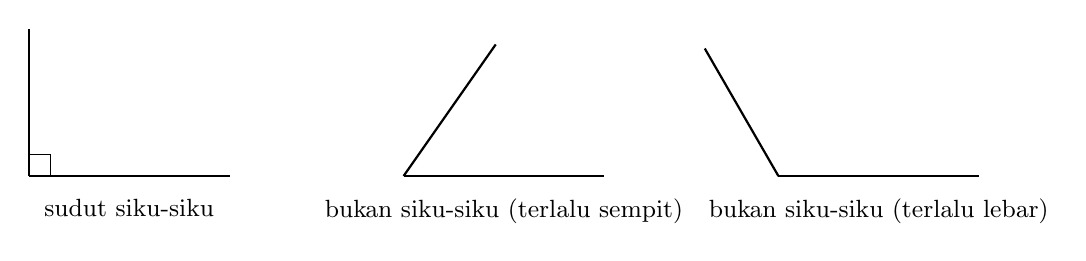
\begin{tikzpicture}[scale=0.85]
  \draw[thick] (0,0) -- (3,0);
  \draw[thick] (0,0) -- (0,2.2);
  \draw[thin] (0.32,0) -- (0.32,0.32) -- (0,0.32);
  \node[below, font=\small] at (1.5,-0.2) {sudut siku-siku};
  \begin{scope}[xshift=5.6cm]
  \draw[thick] (0,0) -- (3,0);
  \draw[thick] (0,0) -- (55:2.4);
  \node[below, font=\small] at (1.5,-0.2) {bukan siku-siku (terlalu sempit)};
  \end{scope}
  \begin{scope}[xshift=11.2cm]
  \draw[thick] (0,0) -- (3,0);
  \draw[thick] (0,0) -- (120:2.2);
  \node[below, font=\small] at (1.5,-0.2) {bukan siku-siku (terlalu lebar)};
  \end{scope}
\end{tikzpicture}

{\small Hanya sudut yang pertama yang siku-siku --- dan hanya tanda
persegi kecil, atau penggaris siku, yang dapat memastikannya: mata
saja mudah tertipu.}
\end{omfigure}

\section{Bangun datar dan aturannya}

\begin{definition}[Persegi, persegi panjang, segitiga]\label{def:g3:shapes:shapes}
\begin{itemize}
  \item \emph{Persegi panjang}\index{persegi panjang} punya $4$ sisi
        dan $4$ \omterm{def:g3:shapes:rightangle}{sudut siku-siku}; sisi-sisi berhadapannya sama panjang.
  \item \emph{Persegi}\index{persegi} adalah persegi panjang yang
        $4$ sisinya sama panjang.
  \item \emph{Segitiga}\index{segitiga} punya $3$ sisi;
        \emph{segitiga siku-siku} punya satu \omterm{def:g3:shapes:rightangle}{sudut siku-siku}.
  \item \emph{Lingkaran}\index{lingkaran} digambar dengan jangka:
        semua titiknya berjarak sama (yaitu \emph{jari-jari}\index{jari-jari})
        dari \emph{pusatnya}.
\end{itemize}
\end{definition}

\begin{omfigure}
\begin{tikzpicture}[scale=0.72]
  % persegi, tanda sudut siku-siku digambar ke arah dalam di setiap pojok
  \draw[thick] (0,0) rectangle (2,2);
  \foreach \x/\y/\dx/\dy in {0/0/1/1, 2/0/-1/1, 0/2/1/-1, 2/2/-1/-1}
    \draw[thin] (\x+0.22*\dx,\y) -- (\x+0.22*\dx,\y+0.22*\dy)
      -- (\x,\y+0.22*\dy);
  \draw (0.93,-0.07) -- (1.07,0.07);
  \draw (0.93,1.93) -- (1.07,2.07);
  \draw (-0.07,0.93) -- (0.07,1.07);
  \draw (1.93,0.93) -- (2.07,1.07);
  \node[below, font=\small] at (1,-0.35) {persegi};
  % persegi panjang
  \begin{scope}[xshift=3.8cm]
  \draw[thick] (0,0) rectangle (3,2);
  \foreach \x/\y/\dx/\dy in {0/0/1/1, 3/0/-1/1, 0/2/1/-1, 3/2/-1/-1}
    \draw[thin] (\x+0.22*\dx,\y) -- (\x+0.22*\dx,\y+0.22*\dy)
      -- (\x,\y+0.22*\dy);
  \node[below, font=\small] at (1.5,-0.35) {persegi panjang};
  \end{scope}
  % segitiga siku-siku
  \begin{scope}[xshift=8.6cm]
  \draw[thick] (0,0) -- (2.6,0) -- (0,2) -- cycle;
  \draw[thin] (0.28,0) -- (0.28,0.28) -- (0,0.28);
  \node[below, font=\small] at (1.3,-0.35) {segitiga siku-siku};
  \end{scope}
  % lingkaran
  \begin{scope}[xshift=13.2cm]
  \draw[thick] (1,1) circle (1.1);
  \fill (1,1) circle (1.5pt);
  \draw[omDef, thick] (1,1) -- ++(45:1.1);
  \node[omDef, font=\small, above right] at (1.72,1.68) {jari-jari};
  \node[below, font=\small] at (1,-0.35) {lingkaran};
  \end{scope}
\end{tikzpicture}

{\small Galeri bangun datar beserta tandanya: persegi kecil untuk
\omterm{def:g3:shapes:rightangle}{sudut siku-siku}, garis kecil untuk sisi yang sama panjang.}
\end{omfigure}

\begin{example}[Mengapa tanda itu penting]\label{ex:g3:shapes:marks}
Bangun yang digambar sedikit miring bisa \emph{terlihat} seperti
persegi tanpa benar-benar menjadi persegi. Tandanyalah yang
mengatakan kebenaran: $4$ tanda \omterm{def:g3:shapes:rightangle}{sudut siku-siku} $+$ $4$ tanda sisi
$=$ persegi yang sungguhan. Ketika menggambar, pasanglah tandanya;
ketika membaca gambar, percayalah hanya pada tanda dan ukuran yang
diberikan.
\end{example}

\section{Menggambar di kertas berpetak}

\begin{method}[Melukis di kertas berpetak]\label{met:g3:shapes:grid}
Kertas berpetak memberi \omterm{def:g3:shapes:rightangle}{sudut siku-siku} secara cuma-cuma: garisnya
saling tegak lurus.
\begin{enumerate}
  \item Untuk menggambar persegi panjang $5$ kali $3$: pilihlah satu
        titik perpotongan, bilanglah $5$ petak ke kanan, $3$ petak ke
        atas, lalu tutuplah bangunnya sepanjang garis petak;
  \item untuk memeriksa panjang yang sama, bilanglah petaknya;
  \item langkah diagonal membuat garis miring: berjalan ``$1$ ke
        kanan, $1$ ke atas'' berulang-ulang menggambar garis
        $45^\circ$.
\end{enumerate}
\end{method}

\begin{omfigure}
\begin{tikzpicture}[scale=0.5]
  \draw[gray!40, thin] (0,0) grid (13,5);
  \draw[very thick, omDef] (1,1) rectangle (6,4);
  \draw[very thick, omThm] (8,1) -- (12,1) -- (8,4) -- cycle;
  \node[omDef, font=\small, below] at (3.5,-0.15)
    {persegi panjang $5 \times 3$};
  \node[omThm, font=\small, below] at (10,-0.15) {segitiga siku-siku};
\end{tikzpicture}

{\small Dua lukisan di kertas berpetak: garis petaknya menjamin
\omterm{def:g3:shapes:rightangle}{sudut siku-sikunya}.}
\end{omfigure}

\begin{example}[Program melukis]\label{ex:g3:shapes:program}
Sebuah gambar dapat dijelaskan dengan langkah bernomor:
``1. Gambarlah persegi $ABCD$ dengan sisi $4$ cm. 2. Gambarlah
lingkaran berpusat $A$ yang melalui $B$.'' Dengan mengikuti program
itu baris demi baris, siapa pun dapat menggambar ulang gambar yang
sama --- dan menuliskannya memaksamu menamai setiap titik. Cobalah
bersama teman: satu menulis, yang lain menggambar.
\end{example}

\section{Latihan}

\begin{exercise}[$\star$]\label{exo:g3:shapes:1}
Di dalam kelas, carilah (tanpa mengukur) tiga \omterm{def:g3:shapes:rightangle}{sudut siku-siku} dan
satu sudut yang bukan siku-siku. Bagaimana kamu \emph{memeriksa} masing-masing?
\end{exercise}

\begin{exercise}[$\star$]\label{exo:g3:shapes:2}
Gambarlah persegi panjang $6$ cm kali $4$ cm dengan penggaris dan
penggaris siku. Tandailah \omterm{def:g3:shapes:rightangle}{sudut siku-siku} dan sisi yang sama panjang.
\end{exercise}

\begin{exercise}[$\star$]\label{exo:g3:shapes:3}
Gambarlah persegi dengan sisi $5$ cm. Berapa \omterm{def:g3:shapes:rightangle}{sudut siku-sikunya}?
Berapa sisi yang sama panjang? Tandailah semuanya.
\end{exercise}

\begin{exercise}[$\star$]\label{exo:g3:shapes:4}
Di kertas berpetak, gambarlah: persegi $4 \times 4$; persegi panjang
$7 \times 2$; segitiga siku-siku dengan sisi siku-siku $3$ dan $5$ petak.
\end{exercise}

\begin{exercise}[$\star$]\label{exo:g3:shapes:5}
Benar atau salah? Jelaskan.
``Setiap persegi adalah persegi panjang.'' \quad
``Setiap persegi panjang adalah persegi.'' \quad
``Sebuah segitiga dapat punya dua \omterm{def:g3:shapes:rightangle}{sudut siku-siku}.'' (Cobalah menggambarnya!)
\end{exercise}

\begin{exercise}[$\star$]\label{exo:g3:shapes:6}
Gambarlah lingkaran dengan \omterm{def:g3:shapes:shapes}{jari-jari} $4$ cm. Tandailah pusatnya $O$,
sebuah titik $A$ pada lingkaran, lalu gambarlah \omterm{def:g3:shapes:shapes}{jari-jari} $[OA]$.
Berapa panjang $OA$? Dan jika $B$ titik lain pada lingkaran itu,
berapa panjang $OB$?
\end{exercise}

\begin{exercise}[$\star$]\label{exo:g3:shapes:7}
Ikutilah program ini: ``1. Gambarlah persegi panjang $ABCD$ dengan
$AB = 6$ cm dan $BC = 3$ cm. 2. Tandailah titik $M$ di tengah
$[AB]$. 3. Hubungkan $M$ ke $C$ dan ke $D$.'' Persegi panjang itu
terpotong menjadi bangun apa saja?
\end{exercise}

\begin{exercise}[$\star$]\label{exo:g3:shapes:8}
Golongkanlah bangun berikut: mana yang punya sedikitnya satu \omterm{def:g3:shapes:rightangle}{sudut
siku-siku}? Persegi; persegi panjang (yang bukan persegi); segitiga
siku-siku; lingkaran; huruf L yang digambar dengan goresan tebal.
\end{exercise}

\begin{exercise}[$\star\star$]\label{exo:g3:shapes:9}
Di kertas berpetak, gambarlah persegi miring yang sisinya berjalan
``$2$ ke kanan, $1$ ke atas'' (beserta belokan yang sesuai).
Bilanglah petaknya untuk meyakinkan dirimu bahwa keempat sisinya sama panjang.
\end{exercise}

\begin{exercise}[$\star\star$]\label{exo:g3:shapes:10}
Tulislah sebuah program melukis (langkah bernomor, titik yang diberi
nama) untuk: persegi dengan sisi $3$ cm yang duduk di atas persegi
panjang $3$ cm $\times$ $2$ cm, seperti rumah di atas lantai
dasarnya. Ujilah programmu pada teman sekelas.
\end{exercise}

\begin{exercise}[$\star\star$]\label{exo:g3:shapes:11}
Berapa banyak persegi yang dapat kamu temukan pada petak
$3 \times 3$ yang tersusun dari persegi kecil? (Bilanglah yang
$1 \times 1$, yang $2 \times 2$ dan yang $3 \times 3$.)

\end{exercise}
